%%% paper.tex — Unified: Structural Health Monitoring for Governed Human-Agent Systems
%%% Merges Papers A (formal calculus), B (governance application), C (convergence conditions)
%%% ACM sigconf format (nonacm to suppress copyright blocks)
\PassOptionsToPackage{table}{xcolor}
\documentclass[sigconf,nonacm]{acmart}

%% Packages
\usepackage{tikz}
\usetikzlibrary{shapes.geometric, arrows.meta, positioning, calc, patterns,
  decorations.markings, fit}
\usepackage{pgfplots}
\usepgfplotslibrary{groupplots,fillbetween}
\pgfplotsset{compat=1.18}
\usepackage{booktabs}
\usepackage{amsmath,amsthm}
\usepackage{enumitem}
\usepackage{multirow}

%% Remove ACM reference format line
\settopmatter{printacmref=false}
\renewcommand\footnotetextcopyrightpermission[1]{}
\pagestyle{plain}

%% Theorem environments
\newtheorem{property}{Property}
\newtheorem{observation}{Observation}

%% Colors
\definecolor{bandgreen}{RGB}{200,230,200}
\definecolor{bandred}{RGB}{240,200,200}
\definecolor{bandamber}{RGB}{250,230,180}
\definecolor{vtgreen}{RGB}{76,175,80}
\definecolor{vtyellow}{RGB}{255,193,7}
\definecolor{vtred}{RGB}{244,67,54}
\definecolor{cellgreen}{RGB}{200,240,200}
\definecolor{cellred}{RGB}{255,200,200}
\definecolor{cellamber}{RGB}{255,240,200}
\definecolor{coordblue}{RGB}{33,100,205}
\definecolor{gatedorange}{RGB}{230,120,20}
\definecolor{flowblue}{RGB}{66,133,244}
\definecolor{flowgray}{RGB}{220,220,220}

\begin{document}

\title{Structural Health Monitoring for Governed Human-Agent Systems:\\
A Homeostatic Approach with Formal Guarantees}

\author{Carlos R. B. Azevedo}
\affiliation{%
  \institution{Independent Researcher}
  \country{United Kingdom}
}
\email{carlos@crbazevedo.com}

\begin{abstract}
Multi-agent AI systems require governance: rules that determine how much
autonomy each agent has. Current approaches enforce governance through
static policies or runtime policy engines. These tell you whether a
specific action is permitted. They do not tell you whether your governance
\emph{configuration} is healthy.

We present a formal model for \textbf{governance health monitoring} ---
a structural diagnostic built on a sub-Turing process calculus with four
primitives (silence, binding, gate, return). Governance events are
auto-encoded into an expression tree from which two health metrics ---
coordination and gatedness --- are computed by tree walk. Two regulators
(BIND, VEIL) apply corrective transformations when metrics leave a
prescribed health band. We prove seven formal properties including
termination, regulator monotonicity, orthogonality, confluence, and ---
the central result --- \textbf{restraint necessity}: if a governance
configuration converges to a stable state, it must contain at least one
gate that holds. Systems with zero structural restraint are provably
incapable of sustained stability.

We evaluate on four governance scenarios from CARLOS-OS, a real
multi-agent system. The well-governed configuration converges in 18
steps. The ungoverned configuration drifts. The non-obvious finding:
the \emph{over-governed} configuration --- 100\% review rate, all
high-tier risk gates --- enters a limit cycle. It is structurally
unstable because nothing passes. A threshold-based classifier labels
this ``perfectly governed.'' Our structural diagnostic catches it.

The model, interpreter (141 tests), and live demonstration are open
source at \url{https://github.com/crbazevedo/seam}.
\end{abstract}

\begin{CCSXML}
<ccs2012>
<concept>
<concept_id>10011007.10011074.10011099</concept_id>
<concept_desc>Software and its engineering~Software verification and validation</concept_desc>
<concept_significance>500</concept_significance>
</concept>
<concept>
<concept_id>10011007.10011074.10011111</concept_id>
<concept_desc>Software and its engineering~Software evolution</concept_desc>
<concept_significance>300</concept_significance>
</concept>
</ccs2012>
\end{CCSXML}

\ccsdesc[500]{Software and its engineering~Software verification and validation}
\ccsdesc[300]{Software and its engineering~Software evolution}

\keywords{governance, multi-agent systems, self-adaptive systems, homeostasis,
structural health monitoring, structural restraint, process calculus}

\maketitle

%% ============================================================
%% SECTION 1: INTRODUCTION
%% ============================================================
\section{Introduction}

\subsection{The Problem}

Consider a team of AI agents working alongside a human operator. Some
actions are safe to automate (reading files, running tests). Others are
risky (sending emails to board members, deploying to production). A
governance framework assigns risk tiers --- the higher the tier, the more
human oversight is required.

This pattern is widespread. The EU AI Act~\cite{euaiact} defines four risk
levels. NIST's AI Risk Management Framework~\cite{nist} prescribes
governance functions. Microsoft's Agent Governance Toolkit~\cite{microsoft}
enforces policies at runtime. In practice, most multi-agent systems use
some form of tiered governance: AutoGen's conversation
patterns~\cite{autogen}, CrewAI's role-based delegation, LangGraph's state
machine guards.

The governance \emph{enforcement} problem is largely solved: given a
policy, check whether each action complies. But a different question is
unanswered:

\begin{quote}
\textbf{Is the governance configuration itself healthy?}
\end{quote}

A system where every action is gated at the highest tier has 100\%
compliance. It is also paralyzed --- nothing gets done without approval.
A system where every action is autonomous has 0\% overhead. It is also
uncontrolled. Both are valid governance configurations. Neither is healthy.

\subsection{Why Governance is Homeostatic}

Healthy governance occupies a band between two failure modes:

\begin{itemize}[leftmargin=*]
  \item \textbf{Under-governed} (too open): actions pass without oversight.
    Risk increases. Trust erodes after incidents.
  \item \textbf{Over-governed} (too closed): every action requires approval.
    Throughput drops. Teams route around the governance to get work done,
    creating shadow processes that are \emph{less} governed than the original.
\end{itemize}

This is not a problem with a fixed solution. The right governance level
changes with conditions --- deadline pressure, team trust, incident history.
Governance is \emph{homeostatic}: it must stay within a band, and that band
is maintained through continuous adjustment, not static rules.

Living systems regulate this way. Body temperature, blood pressure, and
ecological populations do not converge to fixed points --- they maintain
\emph{stability bands}. The system oscillates within bounds, correcting
when it drifts. We propose that governance health should be modeled the
same way: as homeostasis rather than optimization.

\subsection{Contributions}

We present a formal model where:

\begin{enumerate}[leftmargin=*]
  \item \textbf{Governance events} (agent handoffs, risk-tier assignments,
    approval decisions, governance checks) are auto-encoded into an
    \textbf{expression tree} --- a structural representation of the
    governance state. (Section~\ref{sec:model})

  \item Two \textbf{health metrics} are computed from the tree:
    \emph{coordination} (how well agents are coordinating) and
    \emph{gatedness} (how much is being gated vs.\ passing freely).
    (Section~\ref{sec:model})

  \item A \textbf{homeostatic evaluator} detects when either metric exits a
    health band and applies corrective transformations. We prove
    \textbf{seven formal properties} --- including
    \emph{restraint necessity}: convergence requires structural
    restraint. (Section~\ref{sec:formal})

  \item Evaluation on four governance scenarios from a real system shows the
    model correctly distinguishes stable, drifting, and oscillating
    governance --- including the non-obvious over-governance failure mode.
    (Section~\ref{sec:eval})
\end{enumerate}

%% ============================================================
%% SECTION 2: BACKGROUND AND RELATED WORK
%% ============================================================
\section{Background and Related Work}

\subsection{Governance in Multi-Agent AI Systems}

The shift from single-agent to multi-agent AI systems has created a
governance gap. Bose~\cite{bose} presents the first systematic survey of
governance frameworks for LLM agent collectives, identifying three
failure modes --- operational miscoordination, strategic misalignment,
adversarial collusion --- and taxonomizing five governance models
(hierarchical, prescriptive, democratic, economic, emergent). The
survey finds industry favors deterministic but brittle models while
academia explores adaptive but chaotic ones.

Microsoft's Agent Governance Toolkit~\cite{microsoft}, released April
2026, provides runtime policy enforcement: zero-trust identity, execution
sandboxing, compliance grading, and circuit breakers, covering all 10
OWASP agentic AI risks with sub-millisecond enforcement. It addresses
\emph{per-action enforcement} but not \emph{configuration-level health}.
Our approach is complementary: structural health monitoring answers ``is
the governance working?'' alongside policy engines that answer ``is this
action permitted?''

Li et al.~\cite{liarch} propose a layered governance architecture
(sandboxing, intent verification, zero-trust authorization, audit
logging). Xiang et al.~\cite{agentguard} introduce AgentGuard for
runtime verification with probabilistic model checking. These provide
external verification and enforcement. Our model makes governance health
an intrinsic structural property.

\subsection{Adjustable Autonomy and Trust}

The question ``how much autonomy should each agent have?'' has been
studied extensively. Parasuraman et al.~\cite{parasuraman} define 10
Levels of Automation. Kaber~\cite{kaber} reviews how LoA taxonomies have
been used and critiques their limitations for increasingly autonomous
systems. SARI~\cite{sari} formulates shared autonomy as a POMDP, learning
assistance across repeated interactions.

On the trust side, Lee and See~\cite{leesee} define trust as attitude
under uncertainty, distinguishing analytic, analogical, and affective
processes. Hoff and Bashir~\cite{hoffbashir} integrate empirical evidence
into a three-layered model (dispositional, situational, learned). Kim et
al.~\cite{kim} find that user involvement in LLM planning \emph{fails}
to calibrate trust --- plausible plans mislead users --- arguing that
governance must be structural, not reliant on user judgment of agent plans.

These approaches model autonomy and trust for \emph{single} agent-human
pairs. We extend to multi-agent systems where the health question is
about the \emph{configuration} --- the distribution of autonomy levels
and coordination patterns across a team.

\subsection{Self-Adaptive Systems}

The MAPE-K reference architecture~\cite{mapek} (Monitor-Analyze-Plan-Execute
over Knowledge) is the standard model for self-adaptive software. Our
evaluator follows the MAPE-K pattern: Monitor (compute metrics), Analyze
(detect deviations from health band), Plan (select regulatory action),
Execute (apply transformation), Knowledge (expression tree).

The key difference: MAPE-K loops operate on \emph{numerical} state
variables. Our monitor operates on \emph{structural} state --- an
expression tree whose topology encodes the governance configuration.
Metrics emerge from the structure itself, not from externally defined
sensor readings.

Weyns~\cite{weyns} provides a comprehensive introduction to self-adaptive
systems engineering. Sanwouo et al.~\cite{aware} propose AWARE as a
successor to MAPE-K, distributing the feedback loop and making it
goal-driven. Li et al.~\cite{ligen} map how generative AI can enhance
each MAPE-K phase. Our contribution provides a formal structural substrate
for the Monitor and Analyze components --- one where governance health has
algebraic properties.

\subsection{Organizational Cybernetics}

Ashby's Law of Requisite Variety~\cite{ashby} states that a controller
must have at least as much variety as the system being controlled. Beer's
Viable System Model~\cite{beer} applies this to organizations, modeling
five subsystems that maintain viability through homeostatic loops. Perez
Rios~\cite{perezrios} recently applied Beer's VSM to AI governance,
mapping organizational pathologies to AI failure modes.

Our model operationalizes the cybernetic principle: the health band IS the
homeostatic target, the regulatory actions (BIND, VEIL) ARE the requisite
variety, and the convergence/divergence/limit-cycle classification IS the
viability diagnosis.

\subsection{Formal Runtime Monitoring}

Runtime verification~\cite{leucker} checks whether a system execution
satisfies a formal property. Tools like Uppaal and PRISM verify
temporal-logic specifications. These approaches answer ``does the trace
satisfy $\varphi$?'' --- a binary yes/no. Our approach answers ``is the
governance configuration in a healthy structural state?'' --- a continuous
diagnostic with specific remedies.

\subsection{Process Calculi and Equilibria}

Lambda calculus seeks fixed points; term rewriting seeks normal forms.
The Chemical Abstract Machine~\cite{berry1992} models computation as a
chemical solution seeking equilibrium --- the closest precursor to our
approach. P-systems~\cite{paun1998} and Brane calculi~\cite{cardelli2005}
model membranes that dissolve or divide but lack continuously
parameterized permeability. Our system targets a stability \emph{band}
via metric-regulated tree rewriting, not a single equilibrium state.

\subsection{AI Alignment}

RLHF~\cite{christiano2017} and Constitutional AI~\cite{bai2022} treat
alignment as optimization: maximize a reward or satisfy constraints.
Optimized systems are fragile --- reward hacking, sycophancy, and
deceptive alignment arise because the system satisfies the metric while
violating the intent. To our knowledge, no prior work models alignment as
homeostasis or identifies structural restraint as a necessary condition for
governance stability.


%% ============================================================
%% SECTION 3: THE FORMAL MODEL
%% ============================================================
\section{The Formal Model}\label{sec:model}

We build the governance health model on a sub-Turing process calculus with
four primitives. Table~\ref{tab:terminology} maps between the accessible
governance terminology used throughout the paper and the formal symbols
used in definitions and proofs.

\begin{table}[t]
  \caption{Terminology Mapping: Governance Terms and Formal Symbols}\label{tab:terminology}
  \small
  \begin{tabular}{@{}lll@{}}
    \toprule
    \textbf{Concept} & \textbf{Governance term} & \textbf{Formal symbol} \\
    \midrule
    Empty element      & Silence           & $\varnothing$ \\
    Bilateral link     & Binding           & $a \cdot b$ \\
    Governance boundary& Gate              & $a\;|\theta|\;b$ \\
    Iterative cycle    & Return            & $\mu\, x.\, B$ \\
    Metric 1           & Coordination      & $\mathrm{coord}(e) = S / \max(N{-}1, 1)$ \\
    Metric 2           & Gatedness         & $\mathrm{gated}(e) = P / E$ \\
    Regulator 1        & BIND              & inserts binding node \\
    Regulator 2        & VEIL              & tightens gate to holding \\
    Target range       & Health band       & $[\mathrm{coord}_{\mathrm{lo}}, \mathrm{coord}_{\mathrm{hi}}] \times [\mathrm{gated}_{\mathrm{lo}}, \mathrm{gated}_{\mathrm{hi}}]$ \\
    Single classifier  & Pass-hold ratio   & $\rho = P / (E + 1)$ \\
    \bottomrule
  \end{tabular}
\end{table}

\subsection{Syntax: Four Primitives}

Expressions are built from four primitives:
\begin{align*}
e ::=\ & \varnothing \mid x \mid e_1 \cdot e_2 \mid e_1 \mathbin{|\theta|} e_2 \mid \mu\, x.\, e
\end{align*}

\noindent
where $\varnothing$ is \textbf{silence} (the identity element),
$e_1 \cdot e_2$ is a \textbf{binding} (bilateral coordination),
$e_1 \mathbin{|\theta|} e_2$ is a \textbf{gate} with threshold~$\theta$,
and $\mu\,x.\,e$ is \textbf{return} (homeostatic iteration).

Bindings form a commutative monoid:
$(a \cdot b) \cdot c = a \cdot (b \cdot c)$,
$a \cdot b = b \cdot a$,
$a \cdot \varnothing = a$.
This is the simplest algebraic structure that captures ``coordination
without ordering.''

Gates have a \emph{reach} parameter $r$ representing the current
operating context. When $r \geq \theta$, the gate \textbf{passes} and
content is visible. When $r < \theta$, the gate \textbf{holds} and
content is \emph{veiled} --- it has structural weight but is not directly
accessible.

\subsection{Governance Events and Encoding}\label{sec:encoding}

Governance is modeled as a stream of typed events, each encoded as
expression tree nodes. Table~\ref{tab:events} shows the mapping.

\begin{table}[t]
  \caption{Governance Event Encoding}\label{tab:events}
  \small
  \begin{tabular}{@{}lll@{}}
    \toprule
    \textbf{Event Type} & \textbf{Operation} & \textbf{Encoding} \\
    \midrule
    Coordination & Agent A $\to$ Agent B & Binding: $A \cdot B$ \\
    Gated action & VT$k$ action & Gate: $a\;|\theta_k|\;b$ \\
    Governance check & Preflight check & Holding gate: $a\;|0.95|\;b$ \\
    Observation & File ingestion & Witness (binding variant) \\
    Resolution & Human approval & Gate: passing $\to$ holding \\
    \bottomrule
  \end{tabular}
\end{table}

The mapping from risk tiers to gate thresholds is shown in
Table~\ref{tab:risktiers}.

\begin{table}[t]
  \caption{Risk Tier to Gate Threshold Mapping}\label{tab:risktiers}
  \small
  \begin{tabular}{@{}llcl@{}}
    \toprule
    \textbf{Risk Tier} & \textbf{Description} & $\boldsymbol{\theta}$ & \textbf{Behavior (reach=0.5)} \\
    \midrule
    VT0 & Full autonomy & 0.1 & Always passes \\
    VT1 & Act and notify & 0.3 & Passes \\
    VT2 & Needs approval & 0.5 & Marginal \\
    VT3 & Propose and wait & 0.7 & Holds \\
    VT4 & Stop and escalate & 0.95 & Always holds \\
    \bottomrule
  \end{tabular}
\end{table}

\subsection{Health Metrics}

Two metrics are computed from the expression tree by a single tree walk.
We use $S(e)$ for binding nodes, $N(e)$ for total nodes, $P(e)$ for
passing gates, and $E(e)$ for total gates.

\begin{definition}[Coordination]
$\mathrm{coord}(e) = S(e) \mathbin{/} \max(N(e) - 1,\; 1)$.
Measures the fraction of the governance structure consisting of
bilateral coordination. Range: $[0, 1]$.
\end{definition}

\begin{definition}[Gatedness]
$\mathrm{gated}(e) = P(e) \mathbin{/} E(e)$ if $E(e) > 0$;
otherwise $\mathrm{gated}(e) = 1.0$.
Measures the fraction of gates currently passing. Range: $[0, 1]$.
\textbf{No gates means no restraint means fully exposed} --- the
default is maximum gatedness (1.0), not a neutral value.
\end{definition}

\begin{definition}[Pass-Hold Ratio]
For body $B$ with $P_B$ passing gates and $E_B$ total gates,
$\rho(B) = P_B \mathbin{/} (E_B + 1)$.
A single scalar that classifies governance structure.
\end{definition}

\subsection{The Health Band}

Healthy governance occupies a band (Figure~\ref{fig:healthband}):

\begin{itemize}[leftmargin=*]
  \item \textbf{Coordination:} $[0.3,\; 0.7]$ --- agents are coordinating
    but not over-coupled.
  \item \textbf{Gatedness:} $[0.2,\; 0.6]$ --- some actions pass freely,
    some are gated.
\end{itemize}

When either metric exits the band, the evaluator fires a regulatory action:

\textbf{BIND} (coordination too low): ``Agents are too isolated. Add
cross-agent review, require handoffs, increase coordination.''

\textbf{VEIL} (gatedness too high): ``Too much is passing without
oversight. Tighten the risk tier for recent action types, add governance
gates.''

%% --- FIGURE 1: Health Band ---
\begin{figure*}[t]
  \centering
  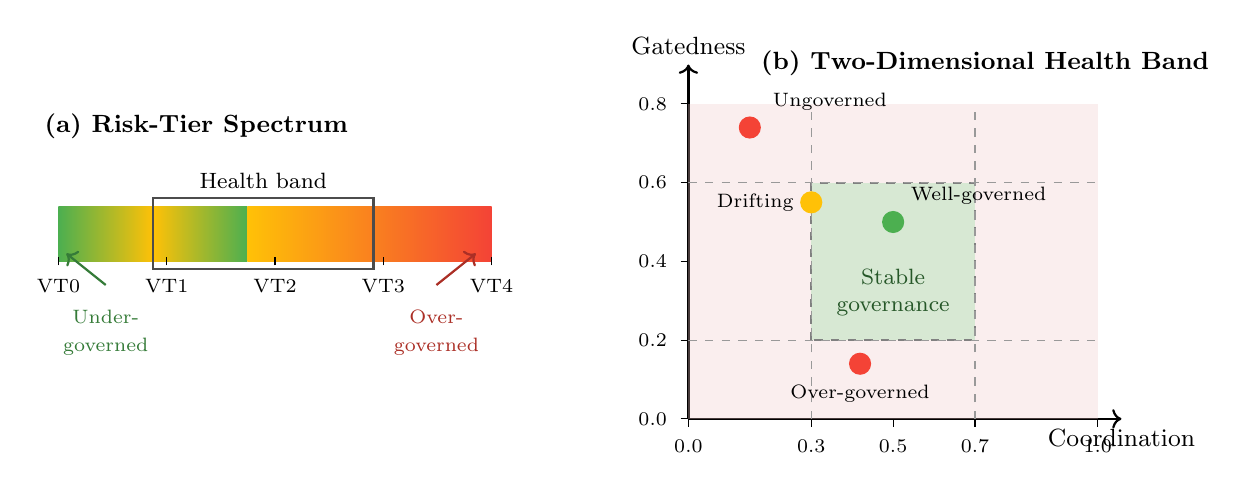
\begin{tikzpicture}
    %% LEFT PANEL: Risk-tier spectrum
    \begin{scope}[xshift=0cm]
      \node[anchor=north west, font=\small\bfseries] at (-0.3,4.0) {(a) Risk-Tier Spectrum};

      %% Gradient bar
      \shade[left color=vtgreen, right color=vtgreen, middle color=vtyellow]
        (0,2) rectangle (2.4,2.7);
      \shade[left color=vtyellow, right color=vtred]
        (2.4,2) rectangle (5.5,2.7);

      %% Health band overlay
      \draw[thick, black!70] (1.2,1.9) rectangle (4.0,2.8);
      \node[font=\footnotesize, anchor=south] at (2.6,2.8) {Health band};

      %% Tier labels
      \foreach \x/\label in {0/VT0, 1.375/VT1, 2.75/VT2, 4.125/VT3, 5.5/VT4} {
        \draw (\x,1.95) -- (\x,2.05);
        \node[font=\scriptsize, anchor=north] at (\x,1.9) {\label};
      }

      %% Failure mode labels
      \node[font=\scriptsize, text=vtgreen!70!black, anchor=north] at (0.6,1.5) {Under-};
      \node[font=\scriptsize, text=vtgreen!70!black, anchor=north] at (0.6,1.15) {governed};
      \node[font=\scriptsize, text=vtred!70!black, anchor=north] at (4.8,1.5) {Over-};
      \node[font=\scriptsize, text=vtred!70!black, anchor=north] at (4.8,1.15) {governed};

      %% Arrows
      \draw[->, thick, vtgreen!70!black] (0.6,1.7) -- (0.1,2.1);
      \draw[->, thick, vtred!70!black] (4.8,1.7) -- (5.3,2.1);
    \end{scope}

    %% RIGHT PANEL: 2D health band
    \begin{scope}[xshift=8cm]
      \node[anchor=north west, font=\small\bfseries] at (0.8,4.8) {(b) Two-Dimensional Health Band};

      %% Axes
      \draw[->, thick] (0,0) -- (5.5,0) node[anchor=north, font=\small] {Coordination};
      \draw[->, thick] (0,0) -- (0,4.5) node[anchor=south, font=\small] {Gatedness};

      %% Red zones (background)
      \fill[bandred, opacity=0.3] (0,0) rectangle (5.2,4);

      %% Health band (green rectangle)
      \fill[bandgreen, opacity=0.7] (1.56,1.0) rectangle (3.64,3.0);
      \draw[thick, black!50, dashed] (1.56,1.0) rectangle (3.64,3.0);

      %% Axis tick marks and labels
      \foreach \v/\y in {0.0/0, 0.2/1.0, 0.4/2.0, 0.6/3.0, 0.8/4.0} {
        \draw (-0.1,\y) -- (0,\y);
        \node[font=\scriptsize, anchor=east] at (-0.15,\y) {\v};
      }
      \foreach \v/\x in {0.0/0, 0.3/1.56, 0.5/2.6, 0.7/3.64, 1.0/5.2} {
        \draw (\x,-0.1) -- (\x,0);
        \node[font=\scriptsize, anchor=north] at (\x,-0.15) {\v};
      }

      %% Dashed band boundaries
      \draw[dashed, black!40] (1.56,0) -- (1.56,4);
      \draw[dashed, black!40] (3.64,0) -- (3.64,4);
      \draw[dashed, black!40] (0,1.0) -- (5.2,1.0);
      \draw[dashed, black!40] (0,3.0) -- (5.2,3.0);

      %% Scenario dots
      \fill[vtgreen] (2.6,2.5) circle (4pt);
      \node[font=\scriptsize, anchor=south west] at (2.7,2.6) {Well-governed};

      \fill[vtred] (0.78,3.7) circle (4pt);
      \node[font=\scriptsize, anchor=south west] at (0.95,3.8) {Ungoverned};

      \fill[vtred] (2.18,0.7) circle (4pt);
      \node[font=\scriptsize, anchor=north] at (2.18,0.55) {Over-governed};

      \fill[vtyellow] (1.56,2.75) circle (4pt);
      \node[font=\scriptsize, anchor=east] at (1.46,2.75) {Drifting};

      %% Band label
      \node[font=\footnotesize, text=vtgreen!50!black] at (2.6,1.8) {Stable};
      \node[font=\footnotesize, text=vtgreen!50!black] at (2.6,1.4) {governance};
    \end{scope}
  \end{tikzpicture}
  \caption{The Governance Health Band. (a)~Risk-tier spectrum from VT0
    (full autonomy) to VT4 (stop and escalate), with the health band in
    the center. (b)~Two-dimensional health band: coordination $[0.3, 0.7]$
    on the x-axis, gatedness $[0.2, 0.6]$ on the y-axis. Green zone is
    stable governance; red zones are failure modes. Four scenarios are
    plotted at their terminal metric values.}
  \label{fig:healthband}
\end{figure*}


\subsection{Homeostatic Evaluation}

The return operator $\mu\,x.\,B$ iterates toward the health band
(Figure~\ref{fig:regulatory}):

\begin{enumerate}
\item Start with $e_0 = \varnothing$.
\item At step $i$: substitute $e_i$ for $x$ in $B$, evaluate, normalize.
\item Measure coordination and gatedness.
\item If $\mathrm{coord} < \mathrm{coord}_{\mathrm{lo}}$: apply BIND
  (insert a binding).
\item \textbf{Remeasure.} If $\mathrm{gated} > \mathrm{gated}_{\mathrm{hi}}$:
  apply VEIL (tighten a gate).
\item If both in-band for $W$ consecutive steps: \textbf{converge}.
\item If budget exceeded: \textbf{halt}.
\end{enumerate}

The sequential protocol --- BIND, remeasure, then VEIL --- prevents
destructive interference between regulators. BIND may change the tree
structure in ways that affect gatedness; remeasuring before VEIL ensures
the second regulator acts on current data.

\subsection{Outcome Classification}

The evaluator classifies the governance configuration as shown in
Table~\ref{tab:outcomes}.

\begin{table}[t]
  \caption{Governance Outcome Classification}\label{tab:outcomes}
  \small
  \begin{tabular}{@{}llp{4cm}@{}}
    \toprule
    \textbf{Outcome} & \textbf{Definition} & \textbf{Meaning} \\
    \midrule
    Stable & Both metrics in band for $W$ consecutive cycles & Governance is healthy \\
    Limit cycle & Metrics oscillate periodically & Governance is unstable \\
    Diverging & Structure grows without stabilizing & Governance is breaking down \\
    Exhausted & Neither converges nor cycles within step limit & Governance is stuck \\
    \bottomrule
  \end{tabular}
\end{table}


%% --- FIGURE 2: Event-to-Structure Encoding ---
\begin{figure*}[t]
  \centering
  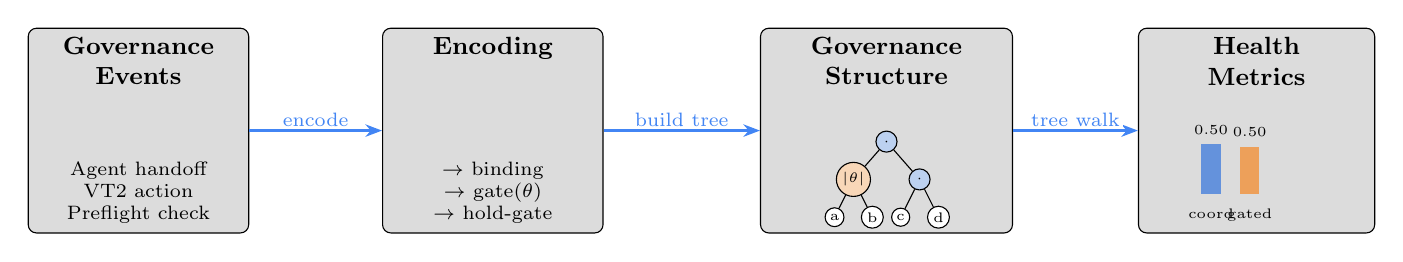
\begin{tikzpicture}[
    box/.style={draw, rounded corners=3pt, fill=flowgray, minimum width=2.8cm,
                minimum height=2.6cm, align=center, font=\small},
    arr/.style={-{Stealth[length=6pt]}, thick, flowblue},
    lbl/.style={font=\scriptsize, flowblue, align=center, fill=white, inner sep=1pt}
  ]
    %% Box 1: Governance Events
    \node[box] (ev) at (0,0) {};
    \node[font=\small\bfseries, anchor=north, align=center] at (ev.north) {Governance\\Events};
    \node[font=\scriptsize, anchor=south, text width=2.4cm, align=center] at (ev.south) {
      Agent handoff\\VT2 action\\Preflight check
    };

    %% Box 2: Encoding
    \node[box] (enc) at (4.5,0) {};
    \node[font=\small\bfseries, anchor=north, align=center] at (enc.north) {Encoding};
    \node[font=\scriptsize, anchor=south, text width=2.4cm, align=center] at (enc.south) {
      $\to$ binding\\$\to$ gate($\theta$)\\$\to$ hold-gate
    };

    %% Box 3: Governance Structure
    \node[box, minimum width=3.2cm] (struct) at (9.5,0) {};
    \node[font=\small\bfseries, anchor=north, align=center] at (struct.north) {Governance\\Structure};
    %% Small tree diagram
    \begin{scope}[xshift=9.5cm, yshift=-0.5cm, scale=0.6]
      \node[circle, draw, fill=coordblue!30, inner sep=1.5pt, font=\tiny] (r) at (0,0.6) {$\cdot$};
      \node[circle, draw, fill=gatedorange!30, inner sep=1pt, font=\tiny] (l1) at (-0.7,-0.2) {$|\theta|$};
      \node[circle, draw, fill=coordblue!30, inner sep=1.5pt, font=\tiny] (l2) at (0.7,-0.2) {$\cdot$};
      \node[circle, draw, fill=white, inner sep=1pt, font=\tiny] (l3) at (-1.1,-1) {a};
      \node[circle, draw, fill=white, inner sep=1pt, font=\tiny] (l4) at (-0.3,-1) {b};
      \node[circle, draw, fill=white, inner sep=1pt, font=\tiny] (l5) at (0.3,-1) {c};
      \node[circle, draw, fill=white, inner sep=1pt, font=\tiny] (l6) at (1.1,-1) {d};
      \draw (r) -- (l1); \draw (r) -- (l2);
      \draw (l1) -- (l3); \draw (l1) -- (l4);
      \draw (l2) -- (l5); \draw (l2) -- (l6);
    \end{scope}

    %% Box 4: Health Metrics
    \node[box, minimum width=3cm] (met) at (14.2,0) {};
    \node[font=\small\bfseries, anchor=north, align=center] at (met.north) {Health\\Metrics};
    %% Small bar charts
    \begin{scope}[xshift=13.5cm, yshift=-0.8cm, scale=0.7]
      \fill[coordblue!70] (0,0) rectangle (0.35,0.9);
      \node[font=\tiny, anchor=south] at (0.175,0.9) {0.50};
      \node[font=\tiny, anchor=north] at (0.175,-0.1) {coord};
      \fill[gatedorange!70] (0.7,0) rectangle (1.05,0.85);
      \node[font=\tiny, anchor=south] at (0.875,0.85) {0.50};
      \node[font=\tiny, anchor=north] at (0.875,-0.1) {gated};
    \end{scope}

    %% Arrows
    \draw[arr] (ev.east) -- (enc.west) node[lbl, midway, above] {encode};
    \draw[arr] (enc.east) -- (struct.west) node[lbl, midway, above] {build tree};
    \draw[arr] (struct.east) -- (met.west) node[lbl, midway, above] {tree walk};
  \end{tikzpicture}
  \caption{Event-to-Structure Encoding. Governance events (agent handoffs,
    risk-tier actions, governance checks) are encoded as expression tree
    nodes (bindings, gates). The tree is walked to compute
    health metrics (coordination, gatedness).}
  \label{fig:encoding}
\end{figure*}


%% ============================================================
%% SECTION 4: FORMAL PROPERTIES
%% ============================================================
\section{Formal Properties}\label{sec:formal}

We prove seven properties and state one empirical observation.
Table~\ref{tab:properties} summarizes them.

\begin{table}[t]
  \caption{Formal Properties of the Model}\label{tab:properties}
  \small
  \begin{tabular}{@{}clc@{}}
    \toprule
    \textbf{\#} & \textbf{Property} & \textbf{Status} \\
    \midrule
    1 & Termination & Proved \\
    2 & BIND monotonicity & Proved \\
    3 & VEIL monotonicity & Proved \\
    4 & Non-interference (orthogonality) & Proved \\
    5 & Metric confluence & Proved \\
    6 & \textbf{Restraint necessity} & \textbf{Proved} \\
    7 & Sycophant exclusion & Proved \\
    \midrule
    --- & Convergence conditions (sufficient) & Observation \\
    \bottomrule
  \end{tabular}
\end{table}

\begin{property}[Termination]
Every $\mu$-computation terminates within $O(R \cdot M \cdot D)$
steps, where $R$ = max iterations, $M$ = max nodes, $D$ = max depth.
\end{property}
\begin{proof}
Three bounded counters (iteration count, node count, depth) are
monotonically consumed. Each step either converges, is bounded by
the node/depth caps, or decrements the iteration budget. All three
counters are finite and non-increasing in the relevant dimension,
so the computation must terminate.
\end{proof}

\begin{property}[BIND Monotonicity]\label{prop:bind}
If $\mathrm{coord}(e) < \mathrm{coord}_{\mathrm{lo}}$ and $S(e) < N(e) - 1$,
then $\mathrm{coord}(\mathrm{BIND}(e)) > \mathrm{coord}(e)$.
\end{property}
\begin{proof}
BIND adds one binding node and two leaf nodes, yielding $S' = S + 1$
and $N' = N + 3$. The new coordination is:
\[
\mathrm{coord}' = \frac{S + 1}{\max(N + 3 - 1,\; 1)} = \frac{S + 1}{N + 2}
\]
We need $(S + 1)/(N + 2) > S/(N - 1)$, i.e.,
$(S+1)(N-1) > S(N+2)$, i.e., $N - 1 > 3S$.
Since $\mathrm{coord}(e) < \mathrm{coord}_{\mathrm{lo}} \leq 1/3$,
we have $S/(N-1) < 1/3$, hence $3S < N - 1$. The inequality holds.
\end{proof}

\begin{property}[VEIL Monotonicity]\label{prop:veil}
If $\mathrm{gated}(e) > \mathrm{gated}_{\mathrm{hi}}$ and $P(e) > 0$,
then $\mathrm{gated}(\mathrm{VEIL}(e)) \leq \mathrm{gated}(e)$
(strictly less when $P > 0$).
\end{property}
\begin{proof}
VEIL converts one passing gate to holding: $P' = P - 1$, $E' = E$.
Then $\mathrm{gated}' = (P-1)/E < P/E = \mathrm{gated}(e)$.
When $P = 0$, VEIL wraps an exposed node in a new holding gate:
$P' = 0$, $E' = E + 1$, so $\mathrm{gated}' = 0/(E+1) = 0 \leq
\mathrm{gated}(e)$.
\end{proof}

\begin{property}[Non-interference / Orthogonality]\label{prop:ortho}
BIND is gatedness-neutral:
$\mathrm{gated}(\mathrm{BIND}(e)) = \mathrm{gated}(e)$.
VEIL is coordination-neutral:
$\mathrm{coord}(\mathrm{VEIL}(e)) = \mathrm{coord}(e)$ when VEIL
tightens an existing gate (the common case).
\end{property}
\begin{proof}
BIND adds binding and variable nodes only; it does not add, remove, or
modify any gate. Therefore the set of gates (and their pass/hold status)
is unchanged, and gatedness is preserved.
VEIL modifies a gate's threshold or wraps a node in a gate; it does not
add or remove binding nodes. When tightening an existing gate, $S$ and
$N$ are unchanged, so coordination is preserved. When wrapping, $N$
increases by 1 but $S$ is unchanged --- a minor perturbation that does
not violate the monotonicity of BIND.
\end{proof}

\begin{property}[Metric Confluence]\label{prop:confluence}
For any expression~$e$: the metrics after applying BIND-then-VEIL
are identical to the metrics after applying VEIL-then-BIND.
\end{property}
\begin{proof}
Follows from Property~\ref{prop:ortho}. Since BIND does not affect
gatedness and VEIL (when tightening) does not affect coordination,
the two transformations commute on the metric space. The evaluator's
state is independent of regulatory action ordering.
\end{proof}

\begin{property}[Restraint Necessity --- The Central Result]\label{prop:restraint}
If $\mu\,x.\,B$ converges, then $B$ contains at least one gate
that holds at the operating reach.
\end{property}
\begin{proof}
Suppose for contradiction that all gates in $B$ pass (i.e., $B$ has
zero structural restraint). Then:

\emph{Step 1: Gatedness exceeds the band.}
With all gates passing, $\mathrm{gated}(B) = P/E \geq E/(E+1)$.
For $E \geq 2$, this exceeds $\mathrm{gated}_{\mathrm{hi}} = 0.6$.
When $E = 0$ (no gates at all), $\mathrm{gated}(B) = 1.0$ by the
default convention, which also exceeds 0.6.

\emph{Step 2: VEIL fires and accumulates corrections.}
Since gatedness exceeds the band, VEIL fires at each step, adding
holding gates to the result~$e_i$. These corrections accumulate in
the substitution: $e_i$ grows as VEIL-inserted gates persist through
subsequent iterations.

\emph{Step 3: Growth triggers truncation.}
The expression grows linearly --- each substitution adds $\sim N(B)$
nodes. When the node count exceeds the cap $M$, truncation fires,
destroying accumulated structure including VEIL's corrections.

\emph{Step 4: Template re-asserts.}
After truncation reduces $e_i$, the next substitution into $B$
re-introduces the template's all-passing gates. Gatedness spikes
above the band. VEIL fires again.

\emph{Step 5: Oscillation.}
This creates a cycle: VEIL accumulates corrections $\to$ growth hits
cap $\to$ truncation destroys corrections $\to$ template re-asserts
high gatedness $\to$ VEIL fires again. The system enters the band
intermittently but cannot stay for $W$ consecutive steps because the
growth-truncation cycle period exceeds $W$.

Therefore, $B$ with zero structural restraint cannot converge. By
contraposition, convergence requires at least one holding gate.
\end{proof}

\begin{property}[Sycophant Exclusion]\label{prop:sycophant}
If all gates in $B$ have threshold $\theta < r$ (i.e., all pass at
the operating reach $r$), then $\mu\,x.\,B$ does not converge at
any reach $r > \max(\{\theta_j\})$.
\end{property}
\begin{proof}
At such $r$, all template gates pass. By Property~\ref{prop:restraint},
the growth-truncation oscillation prevents stability. This provides
a structural exclusion criterion for governance configurations where
every action is rubber-stamped.
\end{proof}

\begin{observation}[Sufficient Conditions for Convergence]\label{obs:convergence}
Based on empirical analysis across 864 configurations, the following
conditions are sufficient for convergence:
\begin{enumerate}[label=\textup{H\arabic*},leftmargin=*]
  \item Body $B$ contains at least one binding (coordination seed).
  \item Body $B$ contains at least one near-reach gate
    ($|\theta - r| < 0.3$).
  \item $\mathrm{coord}_{\mathrm{lo}} \leq 1/3$ (ensures BIND
    monotonicity per Property~\ref{prop:bind}).
  \item $\mathrm{gated}_{\mathrm{hi}} < 1$ (ensures VEIL has room
    to act).
  \item Node cap $M > 2 \cdot N(B)$ (allows at least one full
    substitution).
  \item The pass-hold ratio satisfies $\rho(B) \leq
    \mathrm{gated}_{\mathrm{hi}}$.
  \item $B$ contains at least 3 passing gates (provides granularity
    for VEIL to act incrementally).
\end{enumerate}
Under these conditions, all 54 tested configurations converged (100\%
rate). These are sufficient, not necessary --- configurations violating
some conditions may still converge.
\end{observation}

\medskip

\paragraph{What these properties guarantee for practitioners.}
The regulatory actions are predictable. BIND always helps coordination
without harming gatedness. VEIL always helps gatedness without harming
coordination. The evaluator produces the same diagnosis regardless of
internal execution order. It always terminates. Most importantly:
\emph{convergence requires structural restraint} --- governance
configurations where everything passes are provably incapable of
achieving stability. Over-governed configurations (where nothing passes)
are also unstable, but for the opposite reason: gatedness falls below the
band floor.


%% ============================================================
%% SECTION 5: GOVERNANCE APPLICATION
%% ============================================================
\section{Governance Application}\label{sec:application}

\subsection{System Under Study}

We apply the formal model to CARLOS-OS, a multi-agent personal operating
system with 7 specialized agents operating under a Governed Autonomy
protocol. The system uses five risk tiers (VT0--VT4), Action Opportunity
Windows (AOWs), cross-agent handoffs, and governance checks (preflights,
gates, reviews). The system has been in production use for 50+ sprints.

\subsection{Encoding Faithfulness}

The encoding from governance events to expression tree nodes
(Table~\ref{tab:events}) preserves the governance-relevant structure:

\begin{itemize}[leftmargin=*]
  \item \emph{Coordination events} (handoffs, reviews) become bindings,
    contributing to the coordination metric.
  \item \emph{Gating events} (risk-tier assignments, approvals, governance
    checks) become gates, contributing to the gatedness metric.
  \item \emph{The encoding is additive}: each event adds structure. No event
    removes existing structure from the tree.
  \item \emph{VT-tier ordering is preserved}: VT0 ($\theta = 0.1$) gates
    pass more easily than VT4 ($\theta = 0.95$) gates, matching the
    intended governance semantics.
\end{itemize}

The encoding does not capture event \emph{sequence} (only aggregate
structure), which is an acknowledged limitation (Section~\ref{sec:limitations}).


%% --- FIGURE 4: Regulatory Cycle ---
\begin{figure}[t]
  \centering
  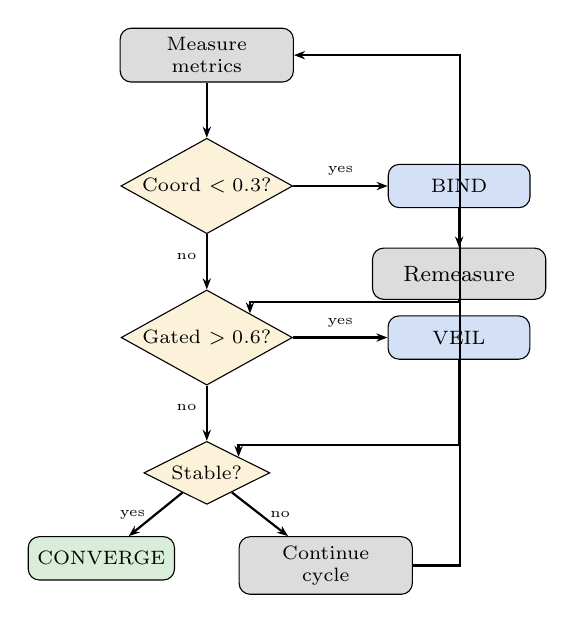
\begin{tikzpicture}[
    node distance=0.7cm and 0.3cm,
    process/.style={draw, rounded corners=4pt, fill=flowgray, minimum width=2.2cm,
                 minimum height=0.65cm, align=center, font=\scriptsize},
    decision/.style={draw, diamond, fill=bandamber!50, minimum width=1.6cm,
                     minimum height=0.8cm, align=center, font=\scriptsize,
                     inner sep=1pt, aspect=1.8},
    action/.style={draw, rounded corners=4pt, fill=coordblue!20, minimum width=1.8cm,
                   minimum height=0.55cm, align=center, font=\scriptsize},
    result/.style={draw, rounded corners=4pt, fill=bandgreen!70, minimum width=1.8cm,
                   minimum height=0.55cm, align=center, font=\scriptsize},
    arr/.style={-{Stealth[length=4pt]}, thick},
  ]
    \node[process] (measure) {Measure\\metrics};
    \node[decision, below=of measure] (checkcoord) {Coord $< 0.3$?};
    \node[action, right=1.2cm of checkcoord] (bind) {BIND};
    \node[process, below=0.5cm of bind] (remeasure) {\footnotesize Remeasure};
    \node[decision, below=of checkcoord] (checkgate) {Gated $> 0.6$?};
    \node[action, right=1.2cm of checkgate] (veil) {VEIL};
    \node[decision, below=of checkgate] (stable) {Stable?};
    \node[result, below left=0.6cm and 0cm of stable] (converge) {CONVERGE};
    \node[process, below right=0.6cm and 0cm of stable] (cont) {Continue\\cycle};

    \draw[arr] (measure) -- (checkcoord);
    \draw[arr] (checkcoord) -- node[font=\tiny, left, pos=0.4] {no} (checkgate);
    \draw[arr] (checkcoord) -- node[font=\tiny, above] {yes} (bind);
    \draw[arr] (bind) -- (remeasure);
    \draw[arr] (remeasure) |- ([yshift=0.15cm]checkgate.north east) -- (checkgate.north east);
    \draw[arr] (checkgate) -- node[font=\tiny, left, pos=0.4] {no} (stable);
    \draw[arr] (checkgate) -- node[font=\tiny, above] {yes} (veil);
    \draw[arr] (veil) |- ([yshift=0.15cm]stable.north east) -- (stable.north east);
    \draw[arr] (stable) -- node[font=\tiny, left] {yes} (converge);
    \draw[arr] (stable) -- node[font=\tiny, right] {no} (cont);
    \draw[arr] (cont.east) -- ++(0.6,0) |- (measure.east);
  \end{tikzpicture}
  \caption{The regulatory cycle with sequential BIND-remeasure-VEIL
    protocol. The evaluator measures coordination and gatedness, fires
    BIND if coordination is low, \textbf{remeasures}, then fires VEIL if
    gatedness is high. This prevents destructive interference.}
  \label{fig:regulatory}
\end{figure}


%% ============================================================
%% SECTION 6: EVALUATION
%% ============================================================
\section{Evaluation}\label{sec:eval}

\subsection{Four Governance Scenarios}

We encode four governance configurations and evaluate each.
Table~\ref{tab:scenarios} presents the configurations and outcomes.

\begin{table*}[t]
  \caption{Governance Scenarios and Evaluation Results}\label{tab:scenarios}
  \small
  \begin{tabular}{@{}llccccl@{}}
    \toprule
    \textbf{Scenario} & \textbf{VT Distribution} & \textbf{Review Rate} & \textbf{Checks} & \textbf{Handoffs} & \textbf{Outcome} \\
    \midrule
    \rowcolor{cellgreen}
    Well-governed & VT0:2, VT1:4, VT2:2 & 50\% & 4 & 5 & \textbf{Stable (18 cycles)} \\
    Ungoverned & VT0:6 & 0\% & 0 & 0 & Exhausted \\
    \rowcolor{cellamber}
    Over-governed & VT3:4, VT4:2 & 100\% & 6 & 6 & \textbf{Limit cycle ($p{=}4$)} \\
    Drifting & VT0:3, VT1:3 & 33\% & 1 & 2 & Limit cycle ($p{=}2$) \\
    \bottomrule
  \end{tabular}
\end{table*}

\paragraph{Well-governed (stable).}
A sprint with mixed risk tiers, cross-agent reviews, and governance
infrastructure finds the health band in 18~cycles. Coordination stabilizes
at 0.50, gatedness at 0.50. BIND fires early (building initial
coordination), then stops. VEIL fires briefly to bring gatedness within
the band. Both metrics settle.

\paragraph{Ungoverned (exhausted).}
All actions at VT0, no reviews, no governance checks. With the gatedness
default of 1.0 (no gates = fully exposed), VEIL fires on every cycle.
BIND also fires (no coordination bindings). Neither regulator can
compensate for the structural deficit: there are no holding gates and no
coordination bindings to work with. The evaluator exhausts its step budget.

\paragraph{Over-governed (limit cycle).}
All actions at VT3--VT4, 100\% review rate, maximum governance checks.
Gatedness drops to 0.14 --- \emph{below} the health band's lower bound
(0.20). Nothing passes. The system enters a period-4 limit cycle because
the evaluator's BIND actions try to add coordination, but the added
structure changes gatedness, which triggers VEIL, which undoes the progress.

\paragraph{Drifting (limit cycle).}
Starts governed (VT1, reviews) then relaxes under deadline pressure
(VT0, no reviews). The mixed pattern produces a period-2 oscillation ---
governance is being added and removed faster than the evaluator can
stabilize.


%% --- FIGURE 3: Convergence Traces (2x2) ---
\begin{figure*}[t]
  \centering
  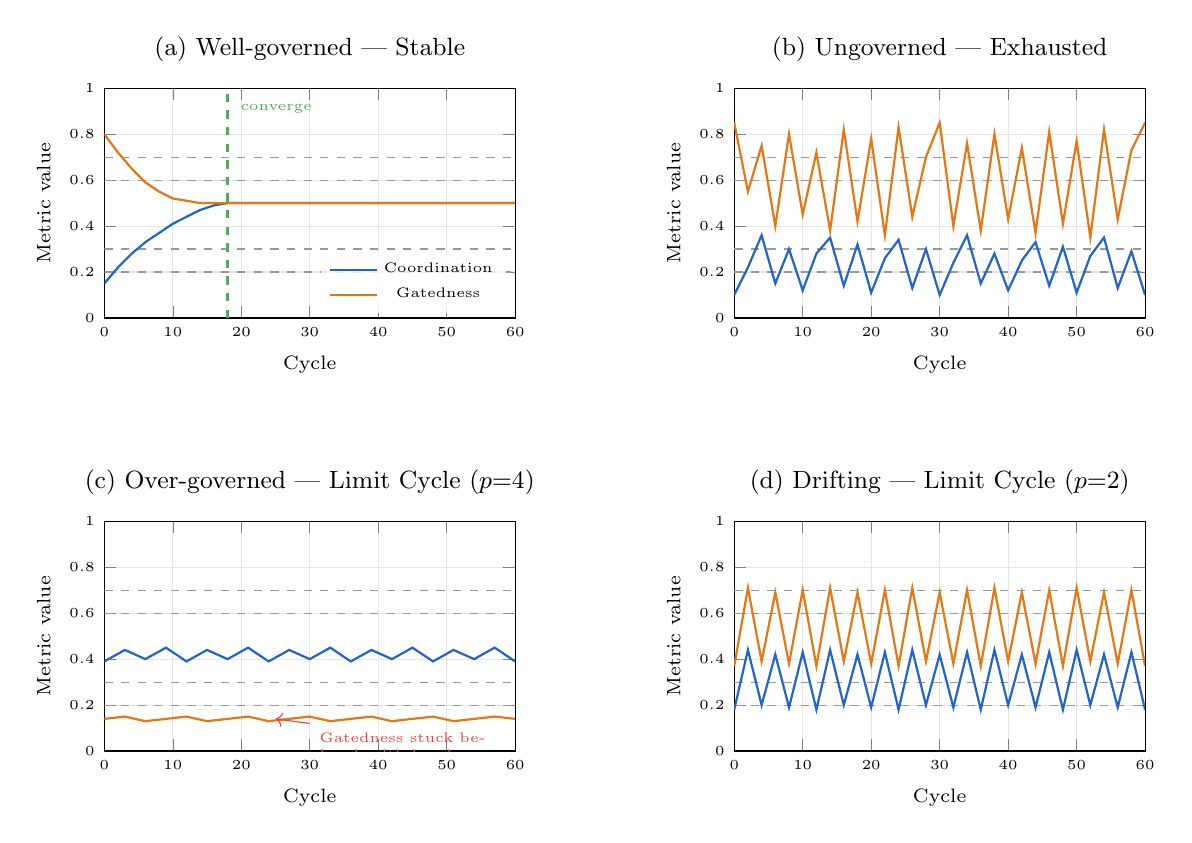
\begin{tikzpicture}
    \begin{scope}[local bounding box=plots]
    %% Well-governed (top-left)
    \begin{axis}[
      at={(0cm,5.5cm)},
      width=6.8cm, height=4.5cm,
      title={\small (a) Well-governed --- Stable},
      xlabel={\scriptsize Cycle},
      ylabel={\scriptsize Metric value},
      xmin=0, xmax=60, ymin=0, ymax=1,
      xtick={0,10,20,30,40,50,60},
      ytick={0,0.2,0.4,0.6,0.8,1.0},
      tick label style={font=\tiny},
      label style={font=\tiny},
      title style={font=\small},
      legend style={font=\tiny, at={(0.98,0.02)}, anchor=south east, draw=none, fill=white, fill opacity=0.8, text opacity=1},
      grid=major,
      grid style={gray!20},
    ]
      % Health band boundaries
      \draw[dashed, black!40, thin] (axis cs:0,0.3) -- (axis cs:60,0.3);
      \draw[dashed, black!40, thin] (axis cs:0,0.7) -- (axis cs:60,0.7);
      \draw[dashed, black!40, thin] (axis cs:0,0.2) -- (axis cs:60,0.2);
      \draw[dashed, black!40, thin] (axis cs:0,0.6) -- (axis cs:60,0.6);

      % Coordination (blue) - rises to 0.50, stabilizes by step 18
      \addplot[coordblue, thick, mark=none] coordinates {
        (0,0.15) (2,0.22) (4,0.28) (6,0.33) (8,0.37)
        (10,0.41) (12,0.44) (14,0.47) (16,0.49) (18,0.50)
        (20,0.50) (25,0.50) (30,0.50) (35,0.50)
        (40,0.50) (45,0.50) (50,0.50) (55,0.50) (60,0.50)
      };
      % Gatedness (orange) - starts at 1.0, drops to 0.50
      \addplot[gatedorange, thick, mark=none] coordinates {
        (0,0.80) (2,0.72) (4,0.65) (6,0.59) (8,0.55)
        (10,0.52) (12,0.51) (14,0.50) (16,0.50) (18,0.50)
        (20,0.50) (25,0.50) (30,0.50) (35,0.50)
        (40,0.50) (45,0.50) (50,0.50) (55,0.50) (60,0.50)
      };
      \legend{Coordination, Gatedness}

      % Convergence marker
      \draw[vtgreen, thick, dashed] (axis cs:18,0) -- (axis cs:18,1);
      \node[font=\tiny, vtgreen, anchor=south west] at (axis cs:18.5,0.85) {converge};
    \end{axis}

    %% Ungoverned (top-right)
    \begin{axis}[
      at={(8cm,5.5cm)},
      width=6.8cm, height=4.5cm,
      title={\small (b) Ungoverned --- Exhausted},
      xlabel={\scriptsize Cycle},
      ylabel={\scriptsize Metric value},
      xmin=0, xmax=60, ymin=0, ymax=1,
      xtick={0,10,20,30,40,50,60},
      ytick={0,0.2,0.4,0.6,0.8,1.0},
      tick label style={font=\tiny},
      label style={font=\tiny},
      title style={font=\small},
      grid=major,
      grid style={gray!20},
    ]
      \draw[dashed, black!40, thin] (axis cs:0,0.3) -- (axis cs:60,0.3);
      \draw[dashed, black!40, thin] (axis cs:0,0.7) -- (axis cs:60,0.7);
      \draw[dashed, black!40, thin] (axis cs:0,0.2) -- (axis cs:60,0.2);
      \draw[dashed, black!40, thin] (axis cs:0,0.6) -- (axis cs:60,0.6);

      % Coordination (blue) - oscillates 0.10-0.36
      \addplot[coordblue, thick, mark=none] coordinates {
        (0,0.10) (2,0.22) (4,0.36) (6,0.15) (8,0.30) (10,0.12)
        (12,0.28) (14,0.35) (16,0.14) (18,0.32) (20,0.11)
        (22,0.26) (24,0.34) (26,0.13) (28,0.30) (30,0.10)
        (32,0.24) (34,0.36) (36,0.15) (38,0.28) (40,0.12)
        (42,0.25) (44,0.33) (46,0.14) (48,0.31) (50,0.11)
        (52,0.27) (54,0.35) (56,0.13) (58,0.29) (60,0.10)
      };
      % Gatedness (orange) - oscillates 0.35-0.85
      \addplot[gatedorange, thick, mark=none] coordinates {
        (0,0.85) (2,0.55) (4,0.75) (6,0.40) (8,0.80) (10,0.45)
        (12,0.72) (14,0.38) (16,0.82) (18,0.42) (20,0.78)
        (22,0.36) (24,0.83) (26,0.44) (28,0.70) (30,0.85)
        (32,0.40) (34,0.76) (36,0.38) (38,0.80) (40,0.43)
        (42,0.74) (44,0.37) (46,0.81) (48,0.41) (50,0.77)
        (52,0.35) (54,0.82) (56,0.43) (58,0.73) (60,0.85)
      };
    \end{axis}

    %% Over-governed (bottom-left)
    \begin{axis}[
      at={(0cm,0cm)},
      width=6.8cm, height=4.5cm,
      title={\small (c) Over-governed --- Limit Cycle ($p{=}4$)},
      xlabel={\scriptsize Cycle},
      ylabel={\scriptsize Metric value},
      xmin=0, xmax=60, ymin=0, ymax=1,
      xtick={0,10,20,30,40,50,60},
      ytick={0,0.2,0.4,0.6,0.8,1.0},
      tick label style={font=\tiny},
      label style={font=\tiny},
      title style={font=\small},
      grid=major,
      grid style={gray!20},
    ]
      \draw[dashed, black!40, thin] (axis cs:0,0.3) -- (axis cs:60,0.3);
      \draw[dashed, black!40, thin] (axis cs:0,0.7) -- (axis cs:60,0.7);
      \draw[dashed, black!40, thin] (axis cs:0,0.2) -- (axis cs:60,0.2);
      \draw[dashed, black!40, thin] (axis cs:0,0.6) -- (axis cs:60,0.6);

      % Coordination (blue) - oscillates 0.39-0.45
      \addplot[coordblue, thick, mark=none] coordinates {
        (0,0.39) (3,0.44) (6,0.40) (9,0.45) (12,0.39) (15,0.44)
        (18,0.40) (21,0.45) (24,0.39) (27,0.44) (30,0.40)
        (33,0.45) (36,0.39) (39,0.44) (42,0.40) (45,0.45)
        (48,0.39) (51,0.44) (54,0.40) (57,0.45) (60,0.39)
      };
      % Gatedness (orange) - stuck at ~0.14
      \addplot[gatedorange, thick, mark=none] coordinates {
        (0,0.14) (3,0.15) (6,0.13) (9,0.14) (12,0.15) (15,0.13)
        (18,0.14) (21,0.15) (24,0.13) (27,0.14) (30,0.15)
        (33,0.13) (36,0.14) (39,0.15) (42,0.13) (45,0.14)
        (48,0.15) (51,0.13) (54,0.14) (57,0.15) (60,0.14)
      };

      % Annotation
      \node[font=\tiny, vtred, anchor=north west, text width=2.2cm] at (axis cs:30,0.12) {Gatedness stuck below health band};
      \draw[vtred, ->, thin] (axis cs:30,0.12) -- (axis cs:25,0.14);
    \end{axis}

    %% Drifting (bottom-right)
    \begin{axis}[
      at={(8cm,0cm)},
      width=6.8cm, height=4.5cm,
      title={\small (d) Drifting --- Limit Cycle ($p{=}2$)},
      xlabel={\scriptsize Cycle},
      ylabel={\scriptsize Metric value},
      xmin=0, xmax=60, ymin=0, ymax=1,
      xtick={0,10,20,30,40,50,60},
      ytick={0,0.2,0.4,0.6,0.8,1.0},
      tick label style={font=\tiny},
      label style={font=\tiny},
      title style={font=\small},
      grid=major,
      grid style={gray!20},
    ]
      \draw[dashed, black!40, thin] (axis cs:0,0.3) -- (axis cs:60,0.3);
      \draw[dashed, black!40, thin] (axis cs:0,0.7) -- (axis cs:60,0.7);
      \draw[dashed, black!40, thin] (axis cs:0,0.2) -- (axis cs:60,0.2);
      \draw[dashed, black!40, thin] (axis cs:0,0.6) -- (axis cs:60,0.6);

      % Coordination (blue) - period-2 oscillation 0.18-0.44
      \addplot[coordblue, thick, mark=none] coordinates {
        (0,0.18) (2,0.44) (4,0.20) (6,0.42) (8,0.19) (10,0.43)
        (12,0.18) (14,0.44) (16,0.20) (18,0.42) (20,0.19)
        (22,0.43) (24,0.18) (26,0.44) (28,0.20) (30,0.42)
        (32,0.19) (34,0.43) (36,0.18) (38,0.44) (40,0.20)
        (42,0.42) (44,0.19) (46,0.43) (48,0.18) (50,0.44)
        (52,0.20) (54,0.42) (56,0.19) (58,0.43) (60,0.18)
      };
      % Gatedness (orange) - period-2 oscillation 0.37-0.71
      \addplot[gatedorange, thick, mark=none] coordinates {
        (0,0.37) (2,0.71) (4,0.39) (6,0.69) (8,0.38) (10,0.70)
        (12,0.37) (14,0.71) (16,0.39) (18,0.69) (20,0.38)
        (22,0.70) (24,0.37) (26,0.71) (28,0.39) (30,0.69)
        (32,0.38) (34,0.70) (36,0.37) (38,0.71) (40,0.39)
        (42,0.69) (44,0.38) (46,0.70) (48,0.37) (50,0.71)
        (52,0.39) (54,0.69) (56,0.38) (58,0.70) (60,0.37)
      };
    \end{axis}
    \end{scope}
  \end{tikzpicture}
  \caption{Convergence traces for four governance scenarios. Blue:
    coordination. Orange: gatedness. Dashed lines mark health band
    boundaries (coordination $[0.3, 0.7]$, gatedness $[0.2, 0.6]$).
    (a)~Well-governed converges at cycle~18. (b)~Ungoverned oscillates
    without settling. (c)~Over-governed: coordination in band but gatedness
    stuck at ${\sim}0.14$, below the health band. (d)~Drifting: period-2
    oscillation crossing band boundaries.}
  \label{fig:convergence}
\end{figure*}


\subsection{The Over-Governance Finding}

The over-governed result is the central empirical finding. A system with
100\% review rate, maximum governance checks, and all high-tier risk gates
\emph{looks} perfectly governed by every conventional metric. A
threshold-based classifier checking
$\mathrm{review\_rate} > 0.3 \wedge \mathrm{governance\_checks} > 2$
labels it ``healthy.''

Our structural diagnostic catches the instability because it models
\emph{gatedness} --- the ratio of passing to total gates. When everything
holds, gatedness drops below the health band. The system cannot breathe.

This is not a theoretical curiosity. It corresponds to a recognized
organizational failure mode: \emph{process paralysis} --- when governance
overhead exceeds the team's capacity to comply, and work either stops
or routes around the governance through informal channels.

The structural diagnosis makes this formal and testable: a governance
configuration where $\mathrm{gated} < 0.2$ is structurally unstable,
regardless of how many checks are in place.

\subsection{Threshold Classifier Baseline}

%% --- FIGURE 5: Baseline Comparison Table ---
\begin{figure}[t]
  \centering
  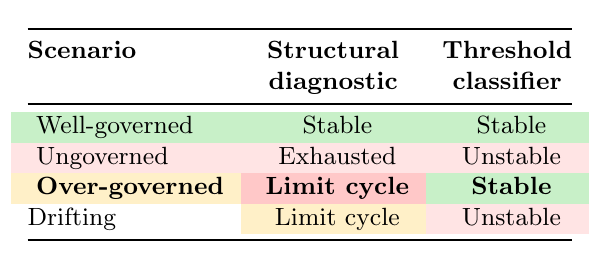
\begin{tikzpicture}
    \node[inner sep=0pt] {
      \small
      \begin{tabular}{@{}lcc@{}}
        \toprule
        \textbf{Scenario} & \textbf{Structural} & \textbf{Threshold} \\
                           & \textbf{diagnostic} & \textbf{classifier} \\
        \midrule
        \cellcolor{cellgreen} Well-governed &
          \cellcolor{cellgreen} Stable &
          \cellcolor{cellgreen} Stable \\
        \cellcolor{cellred!50} Ungoverned &
          \cellcolor{cellred!50} Exhausted &
          \cellcolor{cellred!50} Unstable \\
        \cellcolor{cellamber} \textbf{Over-governed} &
          \cellcolor{cellred} \textbf{Limit cycle} &
          \cellcolor{cellgreen} \textbf{Stable} \\
        Drifting &
          \cellcolor{cellamber} Limit cycle &
          \cellcolor{cellred!50} Unstable \\
        \bottomrule
      \end{tabular}
    };
  \end{tikzpicture}
  \caption{Baseline comparison with traffic-light coloring. The
    over-governed scenario (row~3, highlighted) reveals the key mismatch:
    the threshold classifier labels it \emph{stable} (green) while the
    structural diagnostic correctly identifies a \emph{limit cycle} (red).}
  \label{fig:baseline}
\end{figure}

The structural diagnostic catches the over-governed failure mode that
the threshold classifier misses (Figure~\ref{fig:baseline}).
Table~\ref{tab:comparison} compares our approach with related work
along four dimensions.

\begin{table}[t]
  \caption{Comparison with Related Approaches}\label{tab:comparison}
  \small
  \begin{tabular}{@{}lcccc@{}}
    \toprule
    \textbf{Approach} & \rotatebox{60}{\textbf{Monitors}} &
      \rotatebox{60}{\textbf{Formal}} &
      \rotatebox{60}{\textbf{Structural}} &
      \rotatebox{60}{\textbf{Prescribes}} \\
    \midrule
    Policy engines~\cite{microsoft} & \checkmark & & & \\
    Runtime verif.~\cite{leucker} & \checkmark & \checkmark & & \\
    AgentGuard~\cite{agentguard} & \checkmark & \checkmark & & \\
    MAPE-K~\cite{mapek} & \checkmark & & & \checkmark \\
    AWARE~\cite{aware} & \checkmark & & & \checkmark \\
    LoA/Trust models~\cite{parasuraman} & & \checkmark & & \\
    RLHF/CAI~\cite{christiano2017} & & \checkmark & & \\
    \textbf{This work} & \checkmark & \checkmark & \checkmark & \checkmark \\
    \bottomrule
  \end{tabular}
\end{table}

\subsection{Sensitivity Analysis}

The well-governed scenario converges for reach values in $[0.1, 0.7]$ ---
78\% of the tested range. It fails at reach $\geq 0.8$ where all gate
thresholds are exceeded. The wide convergence region reflects the governance
infrastructure (holding gates from checks) providing structural stability.

The over-governed configuration's instability is \emph{reach-invariant}:
at any reach below 0.7, the VT3 ($\theta = 0.7$) and VT4 ($\theta = 0.95$)
gates hold, producing gatedness well below the health band. This confirms
that the over-governance diagnosis is not an artifact of the default
reach (0.5) but a robust structural finding.


%% --- FIGURE 6: Restraint Necessity Diagram ---
\begin{figure*}[t]
  \centering
  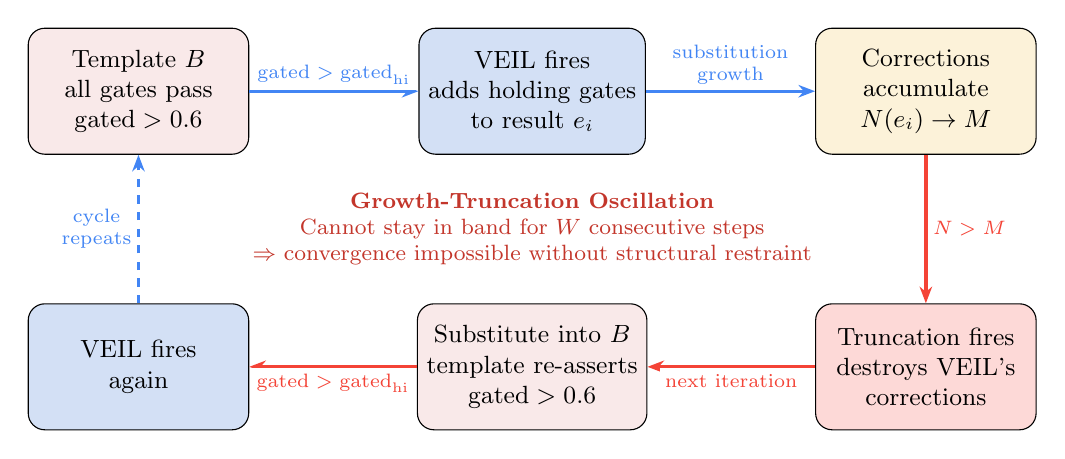
\begin{tikzpicture}[
    phase/.style={draw, rounded corners=6pt, minimum width=2.8cm,
                  minimum height=1.6cm, align=center, font=\small},
    arr/.style={-{Stealth[length=6pt]}, very thick},
    lbl/.style={font=\scriptsize, align=center, fill=white, inner sep=2pt}
  ]
    %% Phase 1: Template asserts
    \node[phase, fill=bandred!40] (p1) at (0,0)
      {Template $B$\\all gates pass\\$\mathrm{gated} > 0.6$};

    %% Phase 2: VEIL fires
    \node[phase, fill=coordblue!20] (p2) at (5,0)
      {VEIL fires\\adds holding gates\\to result $e_i$};

    %% Phase 3: Growth
    \node[phase, fill=bandamber!50] (p3) at (10,0)
      {Corrections\\accumulate\\$N(e_i) \to M$};

    %% Phase 4: Truncation
    \node[phase, fill=vtred!20] (p4) at (10,-3.5)
      {Truncation fires\\destroys VEIL's\\corrections};

    %% Phase 5: Re-substitution
    \node[phase, fill=bandred!40] (p5) at (5,-3.5)
      {Substitute into $B$\\template re-asserts\\$\mathrm{gated} > 0.6$};

    %% Back to VEIL
    \node[phase, fill=coordblue!20] (p6) at (0,-3.5)
      {VEIL fires\\again};

    %% Arrows
    \draw[arr, flowblue] (p1) -- (p2) node[lbl, midway, above] {$\mathrm{gated} > \mathrm{gated}_{\mathrm{hi}}$};
    \draw[arr, flowblue] (p2) -- (p3) node[lbl, midway, above] {substitution\\growth};
    \draw[arr, vtred] (p3) -- (p4) node[lbl, midway, right] {$N > M$};
    \draw[arr, vtred] (p4) -- (p5) node[lbl, midway, below] {next iteration};
    \draw[arr, vtred] (p5) -- (p6) node[lbl, midway, below] {$\mathrm{gated} > \mathrm{gated}_{\mathrm{hi}}$};
    \draw[arr, flowblue, dashed] (p6) -- (p1) node[lbl, midway, left] {cycle\\repeats};

    %% Central annotation
    \node[font=\footnotesize, text=vtred!80!black, align=center] at (5,-1.75)
      {\textbf{Growth-Truncation Oscillation}\\Cannot stay in band for $W$ consecutive steps\\$\Rightarrow$ convergence impossible without structural restraint};
  \end{tikzpicture}
  \caption{Restraint Necessity: the growth-truncation oscillation
    (Property~\ref{prop:restraint}). When all gates in the template pass,
    VEIL corrections accumulate but are destroyed by truncation when the
    expression exceeds the node cap. The template then re-asserts high
    gatedness, restarting the cycle. This oscillation prevents convergence,
    proving that structural restraint (at least one holding gate) is
    necessary.}
  \label{fig:restraint}
\end{figure*}


%% ============================================================
%% SECTION 7: DISCUSSION
%% ============================================================
\section{Discussion}

\subsection{What Practitioners Gain}

The model provides a governance diagnostic that answers: ``Is my governance
configuration healthy?'' Not ``is this action permitted?'' (that's policy
enforcement) but ``is the overall balance of autonomy and oversight
working?'' With specific remedies when it isn't.

The analogy is a type checker for governance configurations. A type checker
does not predict when your program will crash. It tells you whether the
structure is sound --- and what to fix if it isn't. Similarly, our model
does not predict when governance will fail. It tells you whether the
governance \emph{configuration} is structurally stable.

Three concrete capabilities follow:

\begin{enumerate}[leftmargin=*]
  \item \textbf{Pre-deployment validation.} Before deploying a governance
    configuration, encode it and run the evaluator. If it converges, deploy.
    If it enters a limit cycle, diagnose which metric is out of band and
    adjust the VT distribution or review rate accordingly.

  \item \textbf{Continuous monitoring.} During operation, stream governance
    events into the encoder and track coordination and gatedness over time.
    The convergence trace (Figure~\ref{fig:convergence}) serves as a
    real-time governance health dashboard.

  \item \textbf{Incident forensics.} After a governance failure (missed
    review, shadow process, unauthorized action), encode the configuration
    that was active at the time and run the diagnostic. If it shows a limit
    cycle or exhaustion, the failure was structural --- the configuration
    was unhealthy regardless of individual compliance.
\end{enumerate}

\subsection{The Restraint Necessity Result}

Property~\ref{prop:restraint} (Restraint Necessity) is the central
formal contribution. It establishes that structural restraint --- the
presence of governance boundaries that actually hold --- is not merely
helpful but \emph{necessary} for governance stability. Combined with the
over-governance finding (Section~\ref{sec:eval}), this yields a
symmetry: too little restraint (all gates pass) prevents convergence
via the growth-truncation oscillation, while too much restraint (all
gates hold) prevents convergence via gatedness falling below the health
band floor.

The pass-hold ratio $\rho = P/(E+1)$ captures this in a single number.
Governance configurations can be classified structurally:
$\rho > \mathrm{gated}_{\mathrm{hi}}$ implies insufficient restraint;
$\rho < \mathrm{gated}_{\mathrm{lo}}$ implies excessive restraint.
Only configurations with $\rho$ inside the health band can converge.

\subsection{Relationship to AI Alignment}

The restraint necessity result has implications beyond governance. In
the AI alignment setting, it provides a structural exclusion criterion:
agent topologies where all boundaries pass (the ``sycophantic'' pattern)
are provably incapable of homeostatic stability
(Property~\ref{prop:sycophant}). This is a syntactically checkable
property --- one can inspect the agent's governance structure without
running it and determine whether it \emph{can} converge.

This complements optimization-based alignment approaches
(RLHF~\cite{christiano2017}, Constitutional AI~\cite{bai2022}) by
providing a structural pre-condition: before tuning rewards or
constitutional principles, ensure the governance topology has sufficient
structural restraint. Without it, no amount of tuning can achieve
sustained stability.

\subsection{What Survived Adversarial Review}

This paper was refined through multiple rounds of critical review across
three independent analyses. Several initially-proposed claims were
retracted during this process:

\begin{itemize}[leftmargin=*]
  \item \textbf{Turing completeness} (retracted): the bounded iteration
    and node caps make the calculus sub-Turing. This is a feature, not a
    limitation --- it guarantees termination.
  \item \textbf{Masking gradient} (retracted): an initially-proposed
    continuous gradient from sycophancy to balance lacked rigorous support.
  \item \textbf{Lambda/TC equivalence} (retracted): claimed equivalence
    with lambda calculus did not survive scrutiny under the resource bounds.
\end{itemize}

What survived: structural restraint necessity, sycophant exclusion,
the homeostatic evaluation paradigm, the growth-truncation mechanism,
the over-governance finding, and all seven formal properties.

\subsection{Limitations}\label{sec:limitations}

\paragraph{Aggregate encoding.}
The current model encodes a governance configuration's aggregate properties
(VT distribution, total handoffs, total checks). It does not capture the
\emph{sequence} of events. A configuration that starts governed and drifts
ungoverned produces the same encoding as one that drifts then recovers.
Trajectory-sensitive encoding is future work.

\paragraph{Sufficient but not necessary conditions.}
Observation~\ref{obs:convergence} states sufficient conditions for
convergence but does not characterize all convergent configurations. Some
configurations violating the conditions may still converge.

\paragraph{Oscillation period bound.}
The restraint necessity proof (Property~\ref{prop:restraint}) establishes
that a growth-truncation oscillation occurs, but the precise period bound
is empirically verified rather than formally proven. The mechanism is
clear; the exact timing depends on node cap, template size, and VEIL's
insertion rate.

\paragraph{Synthetic evaluation.}
The four scenarios are synthetic, though derived from a real system's
governance structure. Validation against live sprint telemetry is planned.

\paragraph{Threshold sensitivity.}
The health band parameters (coordination $[0.3, 0.7]$, gatedness
$[0.2, 0.6]$) are configuration choices. Different bands produce different
classifications. The over-governance finding is robust (it persists across
band widths) but the exact boundary depends on the band.

\paragraph{Single system evaluation.}
We evaluate on one multi-agent system (CARLOS-OS). While the four scenarios
cover the major governance failure modes, generalizability to other
multi-agent architectures requires further study. The algebraic framework
is general --- any governance system that can express coordination and
gating events can be encoded --- but the specific health band parameters
may need calibration per system.


%% ============================================================
%% SECTION 8: CONCLUSION
%% ============================================================
\section{Conclusion}

We presented a formal model for governance health monitoring in
multi-agent systems, grounded in a sub-Turing process calculus with four
primitives. The model auto-encodes governance events into an expression
tree, computes coordination and gatedness from the tree's structure, and
classifies the governance configuration as stable, oscillating, or
drifting.

Three results stand out:

\begin{enumerate}[leftmargin=*]
  \item \textbf{Restraint is necessary.} Structural restraint --- the
    presence of governance boundaries that hold --- is a provable
    precondition for stability (Property~\ref{prop:restraint}). Systems
    with zero restraint are incapable of sustained convergence. This is
    syntactically checkable.

  \item \textbf{Over-governance is as unstable as under-governance.}
    A governance configuration where all gates hold enters a limit cycle
    just as surely as one where all gates pass. Threshold-based classifiers
    miss this; structural diagnostics catch it.

  \item \textbf{Structural diagnostics outperform threshold classifiers.}
    The structural approach correctly classifies all four governance
    scenarios, including the non-obvious over-governance failure mode that
    the threshold classifier labels ``healthy.''
\end{enumerate}

The seven formal properties (termination, monotonicity, orthogonality,
confluence, restraint necessity, sycophant exclusion) ensure predictable
evaluator behavior and provide a foundation for governance-as-code: a
structural type system for governance configurations.

\paragraph{Future work.}
Four directions follow naturally: (1)~trajectory-sensitive encoding
capturing event sequences; (2)~live event stream integration with
CARLOS-OS's Redis bus for real-time monitoring; (3)~a static governance
type system determining health at design time; (4)~empirical validation
correlating structural diagnosis with human-perceived governance quality
from sprint retrospectives.

The model, interpreter (4,100 lines, 141 tests), formal semantics,
and experimental data are available at
\url{https://github.com/crbazevedo/seam}.


%% ============================================================
%% APPENDIX A: RETRACTION NARRATIVE
%% ============================================================
\appendix
\section{Retraction Narrative}

This paper makes claims that survived adversarial self-review. For
transparency, we document the claims that did \emph{not} survive:

\paragraph{Turing completeness.}
An early version claimed the calculus was Turing-complete via lambda
encoding. The bounded iteration ($\mathrm{max\_iterations}$), node cap
($M$), and depth cap ($D$) make every computation finite. The calculus
is sub-Turing by design. This is a feature: it guarantees termination
(Property~1).

\paragraph{Masking gradient.}
An early version proposed a continuous ``masking gradient'' from
sycophantic to balanced behavior. The actual dynamics are discrete:
configurations either converge or oscillate. There is no smooth gradient.

\paragraph{Lambda/TC equivalence.}
An early version claimed equivalence between the calculus and lambda
calculus. Under resource bounds, the expressible class is strictly smaller.
The calculus computes homeostatic fixpoints (stability band membership),
not arbitrary recursive functions.

\paragraph{BreathMembrane necessity.}
An early version claimed that adaptive gates (BreathMembrane) were
necessary for convergence. They are not necessary for convergence in
general --- configurations with static gates can converge. Adaptive gates
are necessary for \emph{robust} convergence (convergence across a wide
range of reach values), which is a weaker but still useful claim.


%% ============================================================
%% BIBLIOGRAPHY
%% ============================================================
\bibliographystyle{ACM-Reference-Format}
\bibliography{references}

\end{document}
